% Provenance (never printed): see sources/outline_sources.md (Year 2: viscosity, density and
% volatiles of magmas; magma ascent; dykes, sills and plutons; contact aureoles).
% Curves from figdata/bachelor-2/magma.py (GRD 2008 viscosity, DensityX density, Moore 1998
% solubility data, erf sill cooling, Stefan solidification); exercise and problem values in
% the Book 4 scratch calculators calc/ch05.py and calc/ch05pb.py.
\chapter{الصهارات وتموضعها}\label{ch:b2:magma-emplacement}

يجري مصهور بازلتي عند \qty{1200}{\celsius} بلزوجة تقارب
\qty{70}{Pa.s}: ثخين، لكنه ينسكب. أمّا مصهور ريوليتي جاف عند \qty{800}{\celsius}
فلزوجته قرب \qty{e11}{Pa.s}، ولو أُخذت منه كتلة لاحتاجت ساعات كي تتهدّل
تهدّلًا مرئيًا تحت ثقلها. وبين الاثنين عشر رتب من القيمة، أكثر
مما بين الماء والبازلت، ويرجع معظم الفرق إلى أمرين:
السيليكا التي تربط المصهور في شبكة، ودرجة الحرارة،
وهي أدنى بعدّة مئات من الدرجات في الصهارات السيليسية. وبضعة في المئة من
الماء المذاب، وهو ما تستطيع صهارة ريوليتية أن تحمله في العمق، تُخفض لزوجتها
بعامل \num{e5}، ثم تفقد هذا الأثر من جديد حين تصعد \omterm{def:b2:magma-emplacement:magma}{الصهارة} ويخرج
الماء فقاعات. وهذه الأرقام تقرّر هل تبلغ \omterm{def:b2:magma-emplacement:magma}{الصهارة}
السطح بهدوء، أم تنفجر، أم تتجمّد على عمق كيلومترات قاطعًا أو عتبةً أو
بلوتونًا. يعامل هذا الفصل \omterm{def:b2:magma-emplacement:magma}{الصهارة} مادةً: كثافتها ولزوجتها
ومكوّناتها المتطايرة، وفيزياء صعودها عبر الشقوق وعلى هيئة كتل، والأشكال التي
تتّخذها حين تتوقف، والحرارة التي تعطيها للصخور المحيطة بها.
% ledger: grd08:model, grd08:range, moore98:melts

\begin{recall}
\textbf{الجريان اللزج} (مجلد السنة الثانية من كتب الفيزياء): في مائع نيوتني
لزوجته $\eta$ يساوي إجهاد القصّ $\eta$ مضروبة في تدرّج السرعة؛ وبين
جدارين متوازيين يدفع تدرّج الضغط جانبيةً قطعية مكافئة (جريان بوازوي
المستوي)؛ والكرة التي تتحرك ببطء في مائع لزج تخضع لقوة جرّ ستوكس
$6\pi\eta a v$. \textbf{التوصيل الحراري} (المجلد نفسه): تخضع درجة الحرارة للمعادلة
$\partial T/\partial t = \kappa\,\partial^2T/\partial x^2$، مع الانتشارية $\kappa = k/(\rho
c)$، وتنتشر قفزة في درجة الحرارة على هيئة دالة خطأ على مسافة من
رتبة $\sqrt{\kappa t}$. \textbf{الطفو} (مجلد السنة الأولى من كتب الفيزياء): يخضع جسم
مغمور في مائع أكثف منه لقوة صاعدة محصّلة تساوي ثقل المائع
المُزاح ناقصًا ثقله هو. \textbf{التوازن الكيميائي} (كتب الكيمياء): عند
التوازن تحقّق فاعليات النواتج والمتفاعلات قانون فعل
الكتلة بثابت $K$ يتوقف على درجة الحرارة. ومن مجلد السنة الأولى
من هذه السلسلة: الضغط الصخري $p = \rho g z$ والتدرّج الحراري الأرضي؛ ومن
المجلدات المدرسية: الصخور المافية والفلسية، والبلّورات الظاهرة والنُّسُج البورفيرية.
\end{recall}

\section{ما الصهارة}

\begin{definition}[الصهارة]\label{def:b2:magma-emplacement:magma}
\emph{الصهارة}\index{الصهارة} صخر منصهر كليًا أو جزئيًا تحت السطح: أي
\emph{مصهور سيليكاتي}\index{مصهور سيليكاتي}، وهو السائل المكوّن أساسًا من السيليكون
والأكسجين وكاتيونات الفلزات، مع ما يحمله من بلّورات وفقاعات غاز.
و\emph{العجينة البلّورية}\index{العجينة البلّورية} صهارة غنية بالبلّورات إلى حدّ أنها
تتلامس وتكوّن هيكلًا: فلا تستطيع الجريان كسائل، ولا يتحرك مصهورها إلا
عبر المسامّ بين البلّورات.
\end{definition}

يُعطى تركيب المصهور، كما في الصخور، بالنسب المئوية الكتلية
للأكاسيد. وتُتّخذ ثلاثة مصاهير مرجعًا في الفصل كله، وكلها
مدروسة في المختبر: بازلت ثولييتي جُرف من ظهرة وسط محيطية
(نحو \qty{51}{\percent} من SiO$_2$، و\qty{12}{\percent} من أكسيد الحديد، و\qty{7}{\percent}
من MgO)، وأنديزيت (\qty{63}{\percent} من SiO$_2$) وريوليت (\qty{78}{\percent}
من SiO$_2$، و\qty{8}{\percent} من Na$_2$O $+$ K$_2$O وقليل جدًا من الحديد أو المغنيسيوم).
وتختلف درجات حرارة اندفاعها اختلاف تراكيبها: فالصهارات
البازلتية تندفع عند \qtyrange{1000}{1200}{\celsius} (وقد قيست حرارة حمم تجري في أنبوب
على كيلاويا قرب \qty{1200}{\celsius})، والصهارات الأنديزيتية عند
\qtyrange{800}{1000}{\celsius}، والصهارات الريوليتية عند \qtyrange{650}{800}{\celsius}.
\omterm{def:b2:magma-emplacement:magma}{والصهارة} الريوليتية أبرد لأنها بقيّة تبلور طويل
أو أول مصهور من صخور القشرة، وكلاهما يحدث عند درجة حرارة منخفضة
(\cref{ch:b2:magmatic-differentiation}).
% ledger: moore98:melts, tulane:magma-types, earle:kilauea-lava

محتوى البلّورات هو الذي يقرّر هل تجري \omterm{def:b2:magma-emplacement:magma}{الصهارة}. فالدراسات الحقلية والجيوكرونولوجية
لأجسام الغرانيت الكبيرة تخلص إلى أن الجريان الصهاري الكلي يحتاج إلى حصّة
مصهور لا تقل عن \qtyrange{30}{50}{\percent} حجمًا؛ وتحت ذلك تلتحم
البلّورات بجاراتها وتتشوّه المادة كجسم صلب ذي مسامّ
مملوءة بالمصهور. ويُظنّ أن كثيرًا من \omterm{def:b2:magma-emplacement:magma}{الصهارة} المخزّنة في القشرة يقبع في
هذه الحالة، عجينةً تعود متحرّكة حين تُضاف إليها صهارة ساخنة من
الأسفل.
% ledger: glazner04:tuolumne

\section{الكثافة واللزوجة}

\subsection{كثافة المصهور}

ليس \omterm{def:b2:magma-emplacement:magma}{للمصهور السيليكاتي} شبكة بلّورية، لكن حجمه يمكن مع ذلك أن يُبنى من
مكوّناته. فالتجارب على مصاهير كثيرة تُظهر أن كل أكسيد يسهم بحجم
شبه ثابت للمول، هو حجمه المولي الجزئي، الذي يتغيّر ببطء
وخطيًا مع درجة الحرارة والضغط؛ وحجم المصهور هو مجموع
هذه الإسهامات. ويعطي الجدول أدناه القيم المستعملة في هذا الفصل.

\begin{table}[ht]
\centering\small
\begin{tabular}{lrrr}
\hline
الأكسيد & \mbox{\textdir TLT $\bar V_i$ (\unit{cm^3/mol})} & \mbox{\textdir TLT $\partial\bar V_i/\partial T$ (\num{e-3}\,\unit{cm^3/(mol.K)})} & \mbox{\textdir TLT $\partial\bar V_i/\partial p$ (\num{e-4}\,\unit{cm^3/(mol.bar)})} \\
\hline
\mbox{\textdir TLT SiO$_2$}  & 26.86 & 0     & $-1.89$ \\
\mbox{\textdir TLT Al$_2$O$_3$} & 37.42 & 2.62 & $-2.26$ \\
FeO      & 12.68 & 3.69  & $-0.45$ \\
MgO      & 12.02 & 3.27  & $0.27$ \\
CaO      & 16.90 & 3.74  & $0.34$ \\
Na$_2$O  & 29.65 & 7.68  & $-2.40$ \\
K$_2$O   & 47.28 & 12.08 & $-6.75$ \\
H$_2$O   & 22.9  & 9.5   & $-3.20$ \\
\hline
\end{tabular}
\caption{الأحجام المولية الجزئية لمكوّنات الأكاسيد في المصاهير السيليكاتية عند
\qty{1}{bar}، مع مشتقاتها بالنسبة إلى درجة الحرارة والضغط. درجة الحرارة المرجعية
\qty{1773}{K} (\qty{1723}{K} لأكسيد FeO، و\qty{1273}{K} للماء H$_2$O). البيانات:
مجموعة قيم برنامج DensityX (إياكوفينو وتيل، 2019).}
\label{tab:b2:magma-emplacement:volumes}
\end{table}
% ledger: densityx:volumes

\begin{proposition}[كثافة المصهور السيليكاتي]\label{prop:b2:magma-emplacement:density}
ليحوِ مصهورٌ مكوّناتٍ أكسيدية $i$ كسورها المولية $X_i$، وكتلها المولية
$M_i$ وأحجامها المولية الجزئية $\bar V_i(T, p) = \bar V_i^{\circ} + (\partial\bar
V_i/\partial T)(T - T_{\mathrm{ref}}) + (\partial\bar V_i/\partial p)(p - p_{\mathrm{ref}})$.
إذا امتزجت المكوّنات امتزاجًا مثاليًا في الحجم، فإن
\[
\rho = \frac{\sum_i X_i M_i}{\sum_i X_i \bar V_i(T,p)}.
\]
\end{proposition}

\begin{proof}
يحوي مول من المصهور $X_i$ مولًا من المكوّن $i$، كتلتها $X_iM_i$. والامتزاج
المثالي في الحجم يعني أن كل مول من المكوّن $i$ يضيف الحجم $\bar V_i$
أيًّا كانت المكوّنات الأخرى، فيشغل مول المصهور $\sum_i X_i\bar V_i$.
والكثافة هي نسبة الاثنين.
\end{proof}

كتلة الماء المولية \qty{18}{g/mol} فقط، لكن حجمه المولي الجزئي
\qty{22.9}{cm^3/mol}، قريب من حجم السيليكا: فهو يُخفض كثافة المصهور
بشدّة. وبتطبيق القضية على المصاهير المرجعية الثلاثة نحصل على
\qty{2730}{kg/m^3} للبازلت عند \qty{1200}{\celsius}، و\qty{2480}{kg/m^3}
للأنديزيت عند \qty{1000}{\celsius}، و\qty{2340}{kg/m^3} للريوليت الجاف
عند \qty{850}{\celsius}؛ ويُنقص واحد في المئة من الماء المذاب نحو
\qty{70}{kg/m^3} من كثافة البازلت، أي قدر ما تُنقصه عدّة مئات من درجات التسخين.
فالمصهور البازلتي إذن أخفّ من بيريدوتيت الوشاح الذي ينشأ منه
(نحو \qty{3380}{kg/m^3} تحت القشرة في النموذج المرجعي للأرض) وأخفّ
قليلًا من القشرة السفلى في ذلك النموذج (\qty{2900}{kg/m^3})، في حين أن
المصهور الريوليتي أخفّ حتى من قشرته العليا (\qty{2600}{kg/m^3}). وهذا الفرق يدفع الصهارات
إلى الأعلى.
% ledger: densityx:volumes, densityx:water, data:prem

\subsection{اللزوجة}

تحدّد لزوجةَ \omterm{def:b2:magma-emplacement:magma}{المصهور السيليكاتي} شبكةُ رباعيات الأوجه SiO$_4$
المترابطة عبر ذرّات أكسجين مشتركة: فلكي يجري، يجب على المصهور أن يكسر روابط
السيليكون والأكسجين ويعيد تكوينها. فالسيليكا والألومينا تبنيان الشبكة؛ وكاتيونات
المغنيسيوم والحديد والكالسيوم والفلزات القلوية تكسرها، وكذلك الماء الذي
يحوّل ذرّات الأكسجين الجسرية إلى مجموعات هيدروكسيل. وتغطي القياسات المخبرية على
المصاهير الطبيعية أكثر من خمس عشرة رتبة من القيمة، من \qty{0.1}{Pa.s} إلى
\qty{e14}{Pa.s}، ولا تتبع قانون أرهينيوس بسيطًا: فاللزوجة
تزداد أسرع من الأسّي في $1/T$ كلما برد المصهور نحو انتقاله
الزجاجي.
% ledger: grd08:range

\begin{proposition}[قانون فوغل وفولشر وتامّان]\label{prop:b2:magma-emplacement:vft}
تتبع لزوجة \omterm{def:b2:magma-emplacement:magma}{مصهور سيليكاتي} ثابت التركيب، في حدود بضعة
أعشار من الوحدة اللوغاريتمية،
\[
\log_{10}\eta = A + \frac{B}{T - C},
\]
حيث $\eta$ بالباسكال ثانية و$T$ بالكلفن. وفي المصاهير الطبيعية تكون $A$ قريبة
من $-4.55$ أيًّا كان التركيب؛ أمّا $B$ و$C$ (بالكلفن) فتركيبات خطية
من النسب المئوية المولية للأكاسيد، مع بضعة جداءات بينها،
مضبوطة على نحو \num{1800} قياس.
\end{proposition}
\admitted
% ledger: grd08:model, grd08:range

يبيّن الشكل أدناه القانون للمصاهير المرجعية الثلاثة وللريوليت
الحاوي ماءً مذابًا. فعند \qty{1200}{\celsius} تكون للبازلت
$\eta \approx \qty{70}{Pa.s}$؛ وللأنديزيت عند \qty{1000}{\celsius} نحو
\qty{e6}{Pa.s}؛ وللريوليت الجاف عند \qty{800}{\celsius} نحو $10^{10.9}$\,\unit{Pa.s}.
وأربعة في المئة من الماء تُنزل الريوليت نفسه إلى $10^{5.5}$\,\unit{Pa.s}، وستة
في المئة إلى $10^{4.6}$\,\unit{Pa.s}. وتعطي معادلة مستقلة لم تُضبط إلا على المصاهير
الغرانيتية المائية القيمَ نفسها في حدود نصف وحدة لوغاريتمية
(\cref{exo:b2:magma-emplacement:1}). ويبلغ أثر الماء أقصاه عند درجة الحرارة المنخفضة، حيث تغيّر بضعة
أعشار من الواحد في المئة اللزوجةَ برتب من القيمة.
% ledger: grd08:model, hd96:model, moore98:melts

\begin{omfigure}
\centering
\begin{tikzpicture}
\begin{axis}[omrecord, width=0.86\linewidth, height=6.4cm,
  xmin=600, xmax=1400, ymin=0, ymax=15,
  xlabel={\foreignlanguage{arabic}{درجة الحرارة \babelsublr{(\unit{\celsius})}}}, ylabel={\mbox{\textdir TLT $\log_{10}\eta$ (\unit{Pa.s})}},
  legend pos=north east, legend style={font=\scriptsize},
  tick label style={font=\scriptsize}, label style={font=\small}]
\addplot[very thick, black, restrict x to domain=1000:1400] table[x=T_C, y=basalt] {figdata/out/bachelor-2-magma-visc.dat};
\addlegendentry{بازلت جاف}
\addplot[very thick, brown, restrict x to domain=800:1300] table[x=T_C, y=andesite] {figdata/out/bachelor-2-magma-visc.dat};
\addlegendentry{أنديزيت جاف}
\addplot[very thick, red!70!black, restrict x to domain=650:1100] table[x=T_C, y=rhyolite] {figdata/out/bachelor-2-magma-visc.dat};
\addlegendentry{ريوليت جاف}
\addplot[thick, red!70!black, dashed, restrict x to domain=650:1000] table[x=T_C, y=rhy2] {figdata/out/bachelor-2-magma-visc.dat};
\addlegendentry{\foreignlanguage{arabic}{ريوليت، 2 في المئة من H$_2$O}}
\addplot[thick, red!70!black, densely dotted, restrict x to domain=650:1000] table[x=T_C, y=rhy4] {figdata/out/bachelor-2-magma-visc.dat};
\addlegendentry{\foreignlanguage{arabic}{ريوليت، 4 في المئة من H$_2$O}}
\addplot[thick, red!70!black, dashdotted, restrict x to domain=650:1000] table[x=T_C, y=rhy6] {figdata/out/bachelor-2-magma-visc.dat};
\addlegendentry{\foreignlanguage{arabic}{ريوليت، 6 في المئة من H$_2$O}}
\end{axis}
\end{tikzpicture}
\par\smallskip{\small لزوجة المصاهير السيليكاتية بدلالة درجة الحرارة، حسب
قانون فوغل وفولشر وتامّان مع المعاملات المتوقفة على التركيب عند
جوردانو وراسل ودينغويل (2008). البازلت: ثولييت ظهرة وسط محيطية؛
الأنديزيت والريوليت: مصاهير مرجعية مخبرية (مور وآخرون، 1998). ورُسم كل
منحنى على مدى درجات الحرارة التي يمكن أن تكون فيها مثل هذه \omterm{def:b2:magma-emplacement:magma}{الصهارة} منصهرة.}
\end{omfigure}
% ledger: grd08:model, moore98:melts

البلّورات تزيد \omterm{def:b2:magma-emplacement:magma}{الصهارة} صلابة. فمعلّق من جسيمات صلبة يقاوم
القصّ أكثر من سائله وحده، لأن السائل يجب أن يجري حول
الجسيمات، وحين تزدحم الجسيمات حتى تتلامس تنحبس في
هيكل.

\begin{proposition}[علاقة أينشتاين وروسكو]\label{prop:b2:magma-emplacement:roscoe}
لمعلّق يحوي كسرًا حجميًا $\phi$ من الكرات الصلبة في سائل نيوتني
لزوجته $\eta_{\ell}$ لزوجةٌ قدرها
\[
\eta = \eta_{\ell}\,(1 - R\phi)^{-2.5}, \qquad R = 1/\phi_m \approx 1.35,
\]
حيث $\phi_m$ كسر الرصّ الأقصى، الذي ينحشر عنده المعلّق. ومن أجل
$\phi$ الصغيرة تؤول إلى علاقة أينشتاين $\eta = \eta_{\ell}(1 + 2.5\phi)$.
\end{proposition}
\admitted
% ledger: kolz22:einstein-roscoe

عشرون في المئة من البلّورات تضاعف اللزوجة، وأربعون في المئة تضربها في
سبعة، وستون في المئة في أكثر من ستين (\cref{exo:b2:magma-emplacement:5})؛ وفي الصهارات الحقيقية، حيث
البلّورات مستطيلة ومتعدّدة الأحجام، يأتي الانحباس أبكر، قرب
\qtyrange{50}{70}{\percent} من البلّورات، حيث تضع الشواهد الحقلية
نهاية الجريان الكلي.

\section{المكوّنات المتطايرة}

\begin{definition}[المكوّنات الصهارية المتطايرة]\label{def:b2:magma-emplacement:volatiles}
\emph{المكوّن الصهاري المتطاير}\index{المكوّن الصهاري المتطاير} مكوّن من مكوّنات \omterm{def:b2:magma-emplacement:magma}{الصهارة}
يكون مذابًا في المصهور في العمق ويكوّن طورًا غازيًا منفصلًا عند الضغط
المنخفض: أساسًا الماء، ثم ثاني أكسيد الكربون، ثم أنواع الكبريت. و\emph{انفصال
المكوّنات المتطايرة}\index{انفصال المكوّنات المتطايرة} هو خروج مكوّن متطاير من
المصهور إلى فقاعات غاز. و\emph{ضغط الإشباع بالمكوّنات
المتطايرة}\index{ضغط الإشباع بالمكوّنات المتطايرة} لمصهور هو الضغط الذي تتجاوز تحته
مكوّناته المتطايرة المذابة ذوبانيّتها، فلا بدّ أن يتكوّن طور غازي.
\end{definition}

تحمل الصهارات المافية عادة \qtyrange{1}{3}{\percent} من المكوّنات المتطايرة كتلةً،
والصهارات الوسيطة \qtyrange{3}{4}{\percent}، والصهارات الفلسية
\qtyrange{4}{7}{\percent}، وانفصال \qtyrange{4}{6}{\percent} من
الماء هو الذي يدفع معظم الاندفاعات الانفجارية. وتتوقف كمية الماء التي يستطيع المصهور حملها
قبل كل شيء على الضغط. ويبيّن الشكل أدناه قياسات على مصاهير بازلتية
وريوليتية أُبقيت تحت ضغط ماء معلوم حتى تشبّعت، ثم بُرّدت فجأة
لتصير زجاجًا وحُلّلت: تزداد الذوبانية بحدّة عند الضغط المنخفض وببطء
أكبر عند الضغط المرتفع.
% ledger: earle:volatiles, moore98:arc-water, moore98:h2o

\begin{proposition}[قانون الجذر التربيعي للماء]\label{prop:b2:magma-emplacement:sqrt}
لنفترض أن الماء يذوب في \omterm{def:b2:magma-emplacement:magma}{مصهور سيليكاتي} أساسًا على هيئة مجموعات هيدروكسيل، عبر
التفاعل $\mathrm{H_2O\,(gas)} + \mathrm{O^{2-}\,(melt)} \rightleftharpoons
2\,\mathrm{OH^-\,(melt)}$، وأكسجين المصهور بفائض كبير. عندئذ، عند
المحتويات المائية المنخفضة، يتناسب الماء المذاب مع الجذر التربيعي
لضغط الماء: $w \approx s\sqrt{p}$، حيث $s$ ثابت يتوقف على المصهور
ودرجة الحرارة.
\end{proposition}

\begin{proof}
يعطي قانون فعل الكتلة $x_{\mathrm{OH}}^2 = K\,x_{\mathrm{O}}\,f$، حيث $f$
فوغاسية الماء (القريبة من ضغطه عند الضغوط المعتدلة) و$x$
الكسور المولية. وأكسجين المصهور بفائض كبير، فيبقى
$x_{\mathrm{O}}$ شبه ثابت، و$x_{\mathrm{OH}} = \sqrt{Kx_{\mathrm{O}}}\,
\sqrt f$. وكل جزيء ماء مذاب يعطي مجموعتي هيدروكسيل، فيكون الماء المذاب
$x_{\mathrm{OH}}/2$، متناسبًا مع $\sqrt f$. وعند المحتويات الأعلى يذوب جزء
من الماء على هيئة جزيئات، بالتناسب مع $f$ نفسها، فتزداد
الذوبانية أسرع من الجذر التربيعي (\cref{exo:b2:magma-emplacement:10}).
\end{proof}

بضبط $w = s\sqrt p$ على القياسات بطريقة المربعات الصغرى نحصل على
$s = 0.34$ في المئة كتلةً لكل $\sqrt{\unit{MPa}}$ للبازلتات
و$s = 0.44$ للريوليتات؛ وكل قياس يقع في حدود واحد في المئة من
الماء عن منحناه. وعندئذ يكون ضغط الإشباع لمصهور فيه $w$ في المئة
من الماء $p_s = (w/s)^2$: \qty{129}{MPa} لريوليت فيه
\qty{5}{\percent} من الماء، أي نحو \qty{5}{km} في عمق القشرة، لكن
\qty{2}{MPa} فقط لبازلت فيه \qty{0.5}{\percent}، أي مئة متر أو أقل.
% ledger: moore98:h2o

\begin{omfigure}
\centering
\begin{tikzpicture}
\begin{axis}[omrecord, width=0.8\linewidth, height=6cm,
  xmin=0, xmax=300, ymin=0, ymax=9,
  xlabel={\foreignlanguage{arabic}{ضغط الماء \babelsublr{(\unit{MPa})}}}, ylabel={\foreignlanguage{arabic}{الماء المذاب H$_2$O (في المئة كتلةً)}},
  legend pos=south east, legend style={font=\scriptsize},
  tick label style={font=\scriptsize}, label style={font=\small}]
\addplot[very thick, red!70!black] table[x=P_MPa, y=rhyolite] {figdata/out/bachelor-2-magma-solub-fit.dat};
\addlegendentry{\foreignlanguage{arabic}{ريوليت، $0.44\sqrt p$}}
\addplot[only marks, mark=*, mark size=2pt, red!70!black] table[x=P_MPa, y=w] {figdata/out/bachelor-2-magma-solub-rhyolite-data.dat};
\addlegendentry{ريوليت، مقيس}
\addplot[very thick, black] table[x=P_MPa, y=basalt] {figdata/out/bachelor-2-magma-solub-fit.dat};
\addlegendentry{\foreignlanguage{arabic}{بازلت، $0.34\sqrt p$}}
\addplot[only marks, mark=square*, mark size=2pt, black] table[x=P_MPa, y=w] {figdata/out/bachelor-2-magma-solub-basalt-data.dat};
\addlegendentry{بازلت، مقيس}
\end{axis}
\end{tikzpicture}
\par\smallskip{\small ذوبانية الماء في المصاهير البازلتية والريوليتية عند
\qtyrange{800}{1200}{\celsius} بدلالة ضغط الماء: قياسات جمعها
مور وآخرون (1998)، وقوانين جذر تربيعي مضبوطة بالمربعات الصغرى. فعند
\qty{100}{MPa}، أي على عمق نحو \qty{4}{km} في القشرة، يستطيع الريوليت أن يحمل
\qty{4.4}{\percent} من الماء، والبازلت \qty{3.4}{\percent}.}
\end{omfigure}
% ledger: moore98:h2o

ثاني أكسيد الكربون أقل ذوبانًا من الماء بكثير. فهو يذوب على هيئة جزيئات في
الريوليتات وعلى هيئة مجموعات كربونات في البازلتات، وأكثر في المصاهير القلوية منه في
الثولييتات، وتزداد ذوبانيته أيضًا مع الضغط. \omterm{def:b2:magma-emplacement:magma}{فالصهارة} التي تحمل كلا
الغازين تبدأ إذن بالانفصال في العمق، بغاز غني جدًا بثاني أكسيد الكربون CO$_2$، ثم
يغتني الغاز بالماء كلما صعدت \omterm{def:b2:magma-emplacement:magma}{الصهارة}. والبازلتات المندفعة على قاع البحر
العميق تحوي حويصلات فيها أكثر من \qty{95}{\percent} من CO$_2$، وهذا اقتضى
تشبّعًا بغاز CO$_2$ حتى تحت \qty{5}{km} من الماء. وتتراوح تقديرات المحتوى الابتدائي
من CO$_2$ في البازلتات الأم لكيلاويا من \qty{0.2}{\percent} إلى \qty{0.6}{\percent}،
وتسجّل الدخائل المصهورية المحبوسة في بلّورات الأوليفين فيها ضغوط
إشباع تصل إلى \qty{500}{MPa}.
% ledger: lowenstern01:co2, lowenstern01:basalts

يشغل الغاز المنفصل حجمًا كبيرًا. فواحد في المئة من الماء في صهارة عند
\qty{900}{\celsius} يشغل، باعتباره غازًا مثاليًا، نحو \qty{12}{\percent} من
الحجم عند \qty{100}{MPa}، و\qty{57}{\percent} عند \qty{10}{MPa}، وأكثر من
\qty{99}{\percent} عند الضغط الجوي (\cref{exo:b2:magma-emplacement:7}). وتُنقص الفقاعات
كثافة \omterm{def:b2:magma-emplacement:magma}{الصهارة} أكثر وتدفعها إلى الأعلى أسرع؛ وفي \omterm{def:b2:magma-emplacement:magma}{الصهارة} اللزجة
لا تستطيع الإفلات، ويبيّن \cref{ch:b2:eruptive-styles} كيف تفتّتها.

\section{الصعود}

يخضع جسم من \omterm{def:b2:magma-emplacement:magma}{الصهارة} أقل كثافة مما حوله لقوة طفو قدرها
$\Delta\rho\,g$ لوحدة الحجم، حيث $\Delta\rho$ فرق الكثافة. ويستطيع أن
يصعد بطريقتين: عبر شقّ يفتحه أمامه، أو على هيئة كتلة ساخنة
ليّنة تزيح الصخر المحيط جانبًا.

\subsection{القواطع}

في العمق يخضع الصخر لضغط صخري كبير، لكن شقًّا مملوءًا
بصهارة ضغطها أعلى قليلًا من الإجهاد الرئيسي الأصغر يستطيع أن
ينفتح ويستطيل عند طرفه. وتملأ \omterm{def:b2:magma-emplacement:magma}{الصهارة} الشقّ كلما نما، والنتيجة
صفيحة رقيقة من \omterm{def:b2:magma-emplacement:magma}{الصهارة}، عرضها أمتار وطولها كيلومترات، تشقّ طريقها
إلى الأعلى: إنه قاطع في طور التكوّن. ثم تجري \omterm{def:b2:magma-emplacement:magma}{الصهارة} بين جدارين شبه
متوازيين.

\begin{proposition}[جريان الصهارة في قاطع]\label{prop:b2:magma-emplacement:poiseuille}
صهارة نيوتنية لزوجتها $\eta$ يدفعها إلى الأعلى تدرّج ضغط $G$
(في جريان الطفو، $G = \Delta\rho\,g$) بين جدارين متوازيين تفصل بينهما مسافة $w$
تجري بالسرعة المتوسطة
\[
\bar u = \frac{G w^2}{12\,\eta},
\]
وتدفّق الحجم لوحدة طول \omterm{def:b2:magma-emplacement:bodies}{القاطع} هو $q = \bar u w = G w^3/(12\eta)$.
\end{proposition}

\begin{proof}
في الجريان الصفائحي المستقر تكون جانبية السرعة عبر \omterm{def:b2:magma-emplacement:bodies}{القاطع} هي قطع بوازوي
المكافئ المستوي $u(x) = \frac{G}{2\eta}\left(\frac{w^2}{4} - x^2\right)$، من أجل
$-w/2 \le x \le w/2$، الذي ينعدم على الجدارين كليهما. ومتوسطه
$\bar u = \frac1w\int_{-w/2}^{w/2}u\,dx = \frac{G}{2\eta}\left(\frac{w^2}{4} -
\frac{w^2}{12}\right) = \frac{Gw^2}{12\eta}$.
\end{proof}

مكعّب العرض يجعل القواطع العريضة أنجع بكثير من الضيّقة. فبازلت
لزوجته \qty{100}{Pa.s} في قاطع عرضه \qty{1}{m}، مع $\Delta\rho =
\qty{300}{kg/m^3}$، يصعد بنحو \qty{2.5}{m/s} ويعبر \qty{10}{km} من
القشرة في ساعة؛ أمّا ريوليت لزوجته \qty{e6}{Pa.s} في \omterm{def:b2:magma-emplacement:bodies}{القاطع} نفسه فيحتاج إلى أكثر
من سنة، ويتجمّد في الطريق، ولذلك تحتاج الصهارات السيليسية إلى قواطع أعرض بكثير
(\cref{exo:b2:magma-emplacement:6}). وعدد رينولدز $\rho\bar u w/\eta$ لهذه الجريانات
صغير بما يكفي لتبقى صفائحية. ومعدلات الصعود المقدّرة للصهارات
أثناء الاندفاعات تفصل الاندفاعات الانسكابية، تحت نحو \qty{0.1}{m/s}، عن
الانفجارية فوقه، مع مدى انتقالي من \qty{0.005}{m/s} إلى \qty{0.25}{m/s}
يحدث فيه الطرازان كلاهما؛ والكمبرليتات، الآتية من
أعماق تتجاوز \qty{150}{km}، قُدّرت سرعتها من \qty{0.1}{m/s} إلى \qty{30}{m/s}،
وتعطي دراسة انتشار لواحد منها من \qty{0.02}{m/s} إلى \qty{0.23}{m/s} متوسطًا على
آخر \qtyrange{80}{110}{km}، أي رحلة من \numrange{5}{74} يومًا.
% ledger: cassidy18:ascent, casetta23:kimberlite

\subsection{الديابيرات}

\begin{definition}[الديابير، مستوى الطفو المتعادل، الاقتلاع]\label{def:b2:magma-emplacement:ascent}
\emph{الديابير}\index{الديابير} جسم من مادة طافية، صهارة أو صخر منصهر
جزئيًا، يصعد عبر ما يحيط به بإزاحته جانبًا بالجريان.
و\emph{مستوى الطفو المتعادل}\index{مستوى الطفو المتعادل} لصهارة هو
العمق الذي تساوي فيه كثافتها كثافة الصخر المحيط: تحته تكون
\omterm{def:b2:magma-emplacement:magma}{الصهارة} طافية، وفوقه تكون أكثف مما حولها. و\emph{الاقتلاع
الصهاري}\index{الاقتلاع الصهاري} هو انفصال كتل من صخر الجدار أو
السقف، تغوص في \omterm{def:b2:magma-emplacement:magma}{الصهارة}؛ والكتل التي تبقى محصورة في الصخر المتصلّب
هي الصخور الدخيلة (الزينوليثات).
\end{definition}
% ledger: earle:intrusive-bodies

\begin{proposition}[صعود ستوكس]\label{prop:b2:magma-emplacement:stokes}
كرة نصف قطرها $a$ ونقص كثافتها $\Delta\rho$ تصعد ببطء في
وسط نيوتني لزوجته $\eta$ تبلغ السرعة الحدّية
\[
v = \frac{2\,\Delta\rho\,g\,a^2}{9\,\eta}
\]
إن كانت صلبة، و$1.5$ ضعف ذلك إن كانت مائعًا لزوجته مهملة.
\end{proposition}
\admitted

الصخر المحيط \omterm{def:b2:magma-emplacement:ascent}{بالديابير} ليس مائعًا لزوجته \qty{100}{Pa.s}، بل جسم صلب ساخن
لزوجته أعلى برتب كثيرة من القيمة من لزوجة أي مصهور: ففي
القشرة لا تصعد كرة من \omterm{def:b2:magma-emplacement:magma}{الصهارة} قطرها كيلومتر إلا ملّيمترات في السنة،
وتفقد حرارتها قبل أن تصعد بعيدًا بزمن طويل (\cref{exo:b2:magma-emplacement:9}). فالديابيرات
تعمل حيث يكون المحيط ساخنًا ليّنًا، في الوشاح وفي الجذور العميقة
للسلاسل الجبلية، وحيث تكون المادة الطافية كتلة منصهرة جزئيًا
عرضها كيلومترات؛ أمّا القشرة الضحلة فتعبرها القواطع.

\section{التموضع}

معظم \omterm{def:b2:magma-emplacement:magma}{الصهارة} لا يبلغ السطح أبدًا. فهي تتوقف حيث لا تعود طافية،
أو حيث تعترضها طبقة أمتن، وتنتشر في جسم يسجّل شكله
كيف أفسحت لنفسها مكانًا.

\begin{definition}[الأجسام المتداخلة]\label{def:b2:magma-emplacement:bodies}
\emph{البلوتون}\index{البلوتون} كل جسم من \omterm{def:b2:magma-emplacement:magma}{الصهارة} تصلّب داخل
القشرة. و\emph{القاطع}\index{القاطع} بلوتون صفائحي الشكل يقطع
تطبّق الصخر المضيف (أو أي صفيحة إن لم يكن للمضيف تطبّق)؛
و\emph{العتبة}\index{العتبة} بلوتون صفائحي الشكل موازٍ للتطبّق.
و\emph{اللاكوليث}\index{اللاكوليث} عتبة ثخنت بدفع الطبقات
العلوية إلى الأعلى في قبّة. و\emph{الباثوليث}\index{الباثوليث} بلوتون كبير،
أو مجموعة من البلوتونات، مساحة ما يتكشّف منه أكثر من \qty{100}{km^2}.
\end{definition}
% ledger: earle:intrusive-bodies

\begin{omfigure}
\centering
\begin{tikzpicture}[x=1cm, y=1cm, font=\scriptsize]
% layered host
\fill[lith sandstone] (0,4.4) rectangle (12,5.4);
\fill[lith sandstone] (0,4.4) rectangle (12,5.4);
\fill[lith shale] (0,3.3) -- (0,4.4) -- (5.2,4.4) .. controls (5.7,4.95) and (7.0,4.95) .. (7.7,4.4)
  -- (12,4.4) -- (12,3.3) -- cycle;
\draw[thin] (0,4.4) -- (5.2,4.4) .. controls (5.7,4.95) and (7.0,4.95) .. (7.7,4.4) -- (12,4.4);
\fill[lith limestone] (0,2.2) rectangle (12,3.3);
\fill[lith sandstone] (0,0) rectangle (12,2.2);
\draw[thick] (0,0) rectangle (12,5.4);
% batholith at the bottom right
\fill[lith granite] (6.8,0) .. controls (7.2,1.6) and (8.4,2.2) .. (9.6,1.9)
  .. controls (10.6,1.7) and (11.2,1.3) .. (12,1.6) -- (12,0) -- cycle;
\draw[thick] (6.8,0) .. controls (7.2,1.6) and (8.4,2.2) .. (9.6,1.9)
  .. controls (10.6,1.7) and (11.2,1.3) .. (12,1.6);
% aureole around the batholith
\draw[densely dashed, orange!80!black, thick] (6.2,0) .. controls (6.6,2.2) and (8.4,2.8) .. (9.6,2.5)
  .. controls (10.6,2.3) and (11.3,2.0) .. (12,2.2);
% stoped blocks
\fill[lith limestone, draw=black] (8.4,1.0) rectangle (8.8,1.3);
\fill[lith sandstone, draw=black] (10.1,0.7) -- (10.5,0.8) -- (10.4,1.1) -- (10.0,1.0) -- cycle;
% feeder dyke from the bottom left, vertical
\fill[lith basalt] (2.0,0) rectangle (2.35,3.3);
\draw (2.0,0) -- (2.0,3.3) (2.35,0) -- (2.35,3.3);
% sill along shale/limestone contact
\fill[lith basalt] (2.0,3.15) rectangle (5.4,3.45);
\draw (2.0,3.15) -- (5.4,3.15) (2.35,3.45) -- (5.4,3.45);
% laccolith: lens pushing up the shale
\fill[lith basalt] (5.4,3.15) .. controls (5.6,3.95) and (6.6,4.05) .. (7.0,3.9)
  .. controls (7.3,3.8) and (7.4,3.4) .. (7.6,3.15) -- cycle;
\draw (5.4,3.45) .. controls (5.6,3.95) and (6.6,4.05) .. (7.0,3.9)
  .. controls (7.3,3.8) and (7.4,3.4) .. (7.6,3.15) -- (5.4,3.15);
% inclined dyke cutting to the surface from the laccolith
\fill[lith basalt] (6.6,3.95) -- (6.9,3.95) -- (7.6,5.4) -- (7.3,5.4) -- cycle;
% labels
\node[fill=white, fill opacity=0.8, text opacity=1, inner sep=1pt] at (1.2,1.4) {قاطع};
\draw (1.6,1.4) -- (2.0,1.4);
\node[fill=white, fill opacity=0.8, text opacity=1, inner sep=1pt] at (3.6,2.7) {عتبة};
\draw (3.6,2.85) -- (3.6,3.15);
\node[fill=white, fill opacity=0.8, text opacity=1, inner sep=1pt] at (6.2,4.75) {لاكوليث};
\draw (6.2,4.6) -- (6.3,3.95);
\node[fill=white, fill opacity=0.8, text opacity=1, inner sep=1pt] at (9.6,0.5) {باثوليث};
\node[fill=white, fill opacity=0.8, text opacity=1, inner sep=1pt, align=center] at (10.6,3.0) {هالة\\التماس};
\draw (10.6,2.7) -- (10.8,2.3);
\node[fill=white, fill opacity=0.8, text opacity=1, inner sep=1pt, align=left] at (5.0,1.0) {كتل\\مقتلعة};
\draw (5.6,1.0) -- (8.35,1.15);
\end{tikzpicture}
\par\smallskip{\small أشكال الأجسام المتداخلة في صخر مضيف متطبّق (تخطيطي، بلا
مقياس): قاطع مغذٍّ يقطع الطبقات، وعتبة على امتداد سطح تطبّق،
ولاكوليث يقبّب الطبقات فوقه، وقاطع يشقّ طريقه إلى السطح،
وباثوليث مع كتل مقتلعة من سقفه وهالة تماس.}
\end{omfigure}

يتوقف مكان توقّف \omterm{def:b2:magma-emplacement:magma}{الصهارة} أولًا على كثافتها. ففي قشرة تزداد كثافتها
مع العمق تصعد \omterm{def:b2:magma-emplacement:magma}{الصهارة} إلى مستوى طفوها المتعادل وتنتشر
جانبيًا هناك، عتبةً أو عدسة؛ والرسوبيات الخفيفة قرب السطح
مصائد ناجعة على نحو خاص للصهارة البازلتية الكثيفة. ويمكن أيضًا لطبقة متينة صلبة
أن توقف قاطعًا وتحرفه على امتداد قاعدتها. ويبيّن الشكل أدناه
المبدأ.

\begin{omfigure}
\centering
\begin{tikzpicture}[font=\scriptsize]
\begin{axis}[width=0.62\linewidth, height=6cm,
  xmin=0, xmax=1.15, ymin=0, ymax=1, y dir=reverse,
  xtick=\empty, ytick=\empty,
  xlabel={\foreignlanguage{arabic}{الكثافة (تخطيطي)}}, ylabel={\foreignlanguage{arabic}{العمق (تخطيطي)}},
  label style={font=\small}, clip=false]
\addplot[very thick, black, domain=0:1, samples=40] ({0.25 + 0.55*(1 - exp(-3*x))}, {x});
\addplot[very thick, red!70!black] coordinates {(0.62,0) (0.62,1)};
\fill[red!70!black, opacity=0.15] (axis cs:0.62,0.36) rectangle (axis cs:1.15,1);
\draw[densely dashed] (axis cs:0,0.36) -- (axis cs:1.15,0.36);
\node[anchor=south west] at (axis cs:0.02,0.36) {مستوى الطفو المتعادل};
\node[anchor=east, black] at (axis cs:0.46,0.20) {القشرة};
\node[anchor=east, red!70!black] at (axis cs:0.61,0.85) {الصهارة};
\node[anchor=west, align=left] at (axis cs:0.82,0.70) {الصهارة أخفّ:\\تصعد};
\node[anchor=west, align=left] at (axis cs:0.66,0.12) {الصهارة أكثف:\\تتوقف تحته};
\end{axis}
\end{tikzpicture}
\par\smallskip{\small \omterm{def:b2:magma-emplacement:ascent}{مستوى الطفو المتعادل} (تخطيطي). تزداد كثافة
القشرة مع العمق، بانضغاط الرسوبيات وبالانتقال إلى
صخور أكثف؛ وتصعد صهارة ثابتة الكثافة ما دامت أخفّ مما
حولها (المنطقة المظلّلة) وتنتشر حيث تلتقي الكثافتان.}
\end{omfigure}

على \omterm{def:b2:magma-emplacement:bodies}{البلوتون} أن يفسح لنفسه مكانًا. فقد يرفع سقفه، كما يفعل \omterm{def:b2:magma-emplacement:bodies}{اللاكوليث}؛
وقد يدفع جدرانه جانبًا حيث تكون ليّنة؛ وقد يملأ فراغًا فتحه
التصدّع؛ وقد يقتلع سقفه كتلةً كتلة. وطويلًا تُصوِّرت البلوتونات الكبيرة
خزّانات صهارة هائلة تموضعت دفعة واحدة. وقد غيّر التأريخ هذه
الصورة. فبلّورات الزركون في مجموعة تولومني الاندساسية، وهي باثوليث غرانيتي في
كاليفورنيا، تُظهر أنها تموضعت بين \num{95} و\qty{85}{Ma}، الأقدم
عند الحواف والأحدث في المركز، وأن إحدى وحداتها وحدها تموضعت على مدى أكثر
من \qty{3}{Myr}، بين \qty{92.8}{Ma} و\qty{88.8}{Ma}. ولو تموضع جسم واحد من
\omterm{def:b2:magma-emplacement:magma}{الصهارة} سمكه \qty{5}{km} وعرضه \qty{20}{km} على عمق \qty{15}{km} لكان قد
برد تحت \qty{750}{\celsius}، حيث يكون نصفه تقريبًا قد تبلور، في
نحو \num{500000}~سنة. فلا بدّ أن تكون مثل هذه البلوتونات قد تجمّعت تدريجيًا،
من اندساسات أصغر كثيرة كالصفائح والقواطع، على مدى ملايين السنين
(\cref{exo:b2:magma-emplacement:11}).
% ledger: glazner04:tuolumne

\begin{omfigure}
\centering
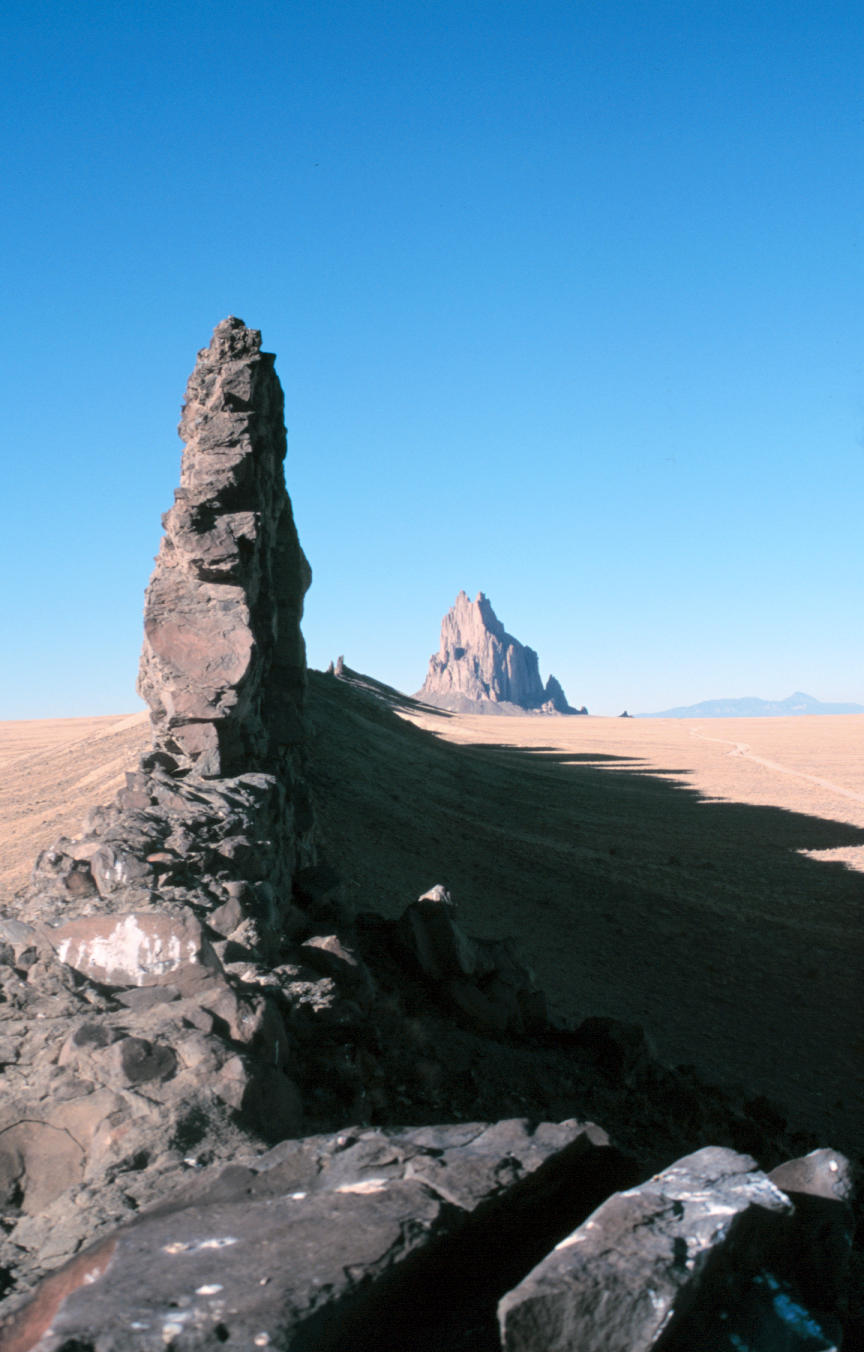
\includegraphics[width=0.3\linewidth]{images/book4/b2-shiprock-dyke.jpg}
\par\smallskip{\small قاطع قرب شيبروك، في حقل نافاهو البركاني
(نيومكسيكو): قاوم صخر \omterm{def:b2:magma-emplacement:bodies}{القاطع} الحتّ أفضل من الحجر الرملي والطفل
اللذين قطعهما، فهو اليوم قائم كالجدار؛ وفي البعيد العنق البركاني الذي
تتشعّع منه عدّة قواطع من هذا النوع. الصورة: \babelsublr{Dexter Perkins (CC0)}.}
\end{omfigure}

\section{التبريد والتحوّل التماسي}

يفقد الجسم المتداخل حرارته بالتوصيل إلى صخوره المضيفة. وأبسط
نموذج يعامل الجسم المتداخل ومضيفه وسطًا موصلًا واحدًا منتظم
الانتشارية $\kappa$: في اللحظة صفر تكون صفيحة سمكها $b$ عند درجة حرارة الجسم
المتداخل $T_m$ والمضيف عند $T_0$. وحلّ معادلة الحرارة، حيث
$x$ مقيسة من منتصف الصفيحة، هو
\[
T(x,t) = T_0 + \frac{T_m - T_0}{2}\left[\operatorname{erf}\frac{b/2 - x}{2\sqrt{\kappa t}}
+ \operatorname{erf}\frac{b/2 + x}{2\sqrt{\kappa t}}\right].
\]
ويبيّن الشكل أدناه هذا الحلّ لعتبة سمكها \qty{100}{m}.
% ledger: delaney86b4:properties

\begin{proposition}[درجة حرارة التماس]\label{prop:b2:magma-emplacement:contact}
في هذا النموذج، ما دام $\sqrt{\kappa t}$ صغيرًا مقارنة بالسمك $b$، تبقى
درجة الحرارة عند تماس الجسم المتداخل مساوية للمتوسط $(T_m + T_0)/2$ لدرجتي حرارة
الجسم المتداخل والمضيف.
\end{proposition}

\begin{proof}
عند التماس $x = b/2$ تكون دالة الخطأ الأولى $\operatorname{erf}0 = 0$
والثانية $\operatorname{erf}(b/(2\sqrt{\kappa t}))$، القريبة من $1$ ما دام
$b \gg 2\sqrt{\kappa t}$. وعندئذ $T = T_0 + (T_m - T_0)/2$.
\end{proof}

فقاطع بازلتي عند \qty{1150}{\celsius} في صخور عند \qty{50}{\celsius} يسخّن إذن
تماسه إلى \qty{600}{\celsius}. وحرارة التبلور، وهي عادة
\qtyrange{700}{1000}{MJ/m^3}، تبقي \omterm{def:b2:magma-emplacement:magma}{الصهارة} ساخنة مدة أطول وترفع هذه القيمة:
فمع \qty{900}{MJ/m^3} محرَّرة بين \num{1150} و\qty{950}{\celsius} يعطي النموذج
نفسه \qty{690}{\celsius}، في حين أن الموصليات المتوقفة على درجة الحرارة والصخور المضيفة
الرطبة تخفض التقديرين كليهما بمقدار 50 إلى \qty{75}{\celsius}.
% ledger: delaney86b4:dike, delaney86b4:properties

\begin{omfigure}
\centering
\begin{tikzpicture}
\begin{axis}[omrecord, width=0.86\linewidth, height=6cm,
  xmin=-200, xmax=200, ymin=0, ymax=1200,
  xlabel={\foreignlanguage{arabic}{البعد عن منتصف العتبة \babelsublr{(\unit{m})}}},
  ylabel={\foreignlanguage{arabic}{درجة الحرارة \babelsublr{(\unit{\celsius})}}},
  legend pos=north east, legend style={font=\scriptsize},
  tick label style={font=\scriptsize}, label style={font=\small}]
\fill[gray!15] (axis cs:-50,0) rectangle (axis cs:50,1200);
\addplot[very thick, red!80!black] table[x=x_m, y=t1] {figdata/out/bachelor-2-magma-sill.dat};
\addlegendentry{بعد سنة واحدة}
\addplot[very thick, orange!90!black] table[x=x_m, y=t2] {figdata/out/bachelor-2-magma-sill.dat};
\addlegendentry{\foreignlanguage{arabic}{بعد 10 سنوات}}
\addplot[very thick, blue!60!black] table[x=x_m, y=t3] {figdata/out/bachelor-2-magma-sill.dat};
\addlegendentry{\foreignlanguage{arabic}{بعد 50 سنة}}
\addplot[very thick, black] table[x=x_m, y=t4] {figdata/out/bachelor-2-magma-sill.dat};
\addlegendentry{\foreignlanguage{arabic}{بعد 200 سنة}}
\draw[densely dashed, gray] (axis cs:-200,625) -- (axis cs:200,625);
\node[font=\scriptsize, gray!40!black, anchor=south west] at (axis cs:-198,625) {$(T_m + T_0)/2$};
\node[font=\scriptsize, anchor=south] at (axis cs:0,20) {العتبة};
\end{axis}
\end{tikzpicture}
\par\smallskip{\small التبريد بالتوصيل لعتبة سمكها \qty{100}{m} (المنطقة المظلّلة)،
اندسّت عند \qty{1150}{\celsius} في صخر عند \qty{100}{\celsius}، مع
$\kappa = \qty{0.7e-6}{m^2/s}$ ودون حرارة كامنة. يبقى التماس قرب
\qty{625}{\celsius} عقودًا بينما تنتشر الحرارة في المضيف؛ وبعد قرنين
تكوّن \omterm{def:b2:magma-emplacement:bodies}{العتبة} ومحيطها نطاقًا دافئًا واحدًا عريضًا.}
\end{omfigure}
% ledger: delaney86b4:properties

السلّم الزمني للتبريد هو الزمن الذي تحتاجه الحرارة لتنتشر عبر
الجسم المتداخل، من رتبة $(b/2)^2/\kappa$: نحو \num{16} يومًا لقاطع
عرضه \qty{2}{m}، وقرن لعتبة سمكها \qty{100}{m}، ومئة ألف سنة
لبلوتون من بضعة كيلومترات. وتطيله الحرارة الكامنة، وكذلك
الحاجة إلى تصليب \omterm{def:b2:magma-emplacement:magma}{الصهارة} لا مجرد تبريدها.

\begin{proposition}[تصلّب جسم متداخل]\label{prop:b2:magma-emplacement:stefan}
لتملأ صهارةٌ عند درجة حرارة تصلّبها $T_m$، وحرارتها الكامنة $L$ لوحدة
الحجم، الحيّزَ $y > 0$ بجوار صخر مضيف عند $T_0$ يشغل $y < 0$، ولكليهما
سعة حرارية $\rho c$ لوحدة الحجم وانتشارية $\kappa$. عندئذ
تتقدّم جبهة التصلّب وفق $y_s = 2\lambda\sqrt{\kappa t}$، حيث $\lambda$
جذر المعادلة
\[
\frac{L\sqrt\pi}{\rho c\,(T_m - T_0)} = \frac{e^{-\lambda^2}}{\lambda\,(1 + \operatorname{erf}\lambda)},
\]
ويبقى التماس عند $T_0 + (T_m - T_0)/(1 + \operatorname{erf}\lambda)$. \omterm{def:b2:magma-emplacement:bodies}{والعتبة}
التي سمكها $b$، وتتصلّب من جداريها كليهما، تصير صلبة بعد
$t = b^2/(16\lambda^2\kappa)$.
\end{proposition}

\begin{proof}
تبقى \omterm{def:b2:magma-emplacement:magma}{الصهارة} أمام الجبهة عند $T_m$، فلا تجري الحرارة إلا في الجزء الصلب
والمضيف، حيث نجرّب $T = T_0 + (T_m - T_0)(1 + \operatorname{erf}\xi)/(1 +
\operatorname{erf}\lambda)$ مع $\xi = y/(2\sqrt{\kappa t})$. وكل دالة في $\xi$
من الشكل $\alpha + \beta\operatorname{erf}\xi$ تحلّ معادلة الحرارة؛ وهذه
تؤول إلى $T_0$ بعيدًا داخل المضيف ($\xi \to -\infty$) وتساوي $T_m$ على الجبهة
$\xi = \lambda$. وعند $y = 0$ تعطي درجة حرارة التماس المذكورة. وعلى الجبهة
يجب أن تُنقل بعيدًا الحرارة الكامنة التي يحرّرها الجزء الصلب المتقدّم، $L\,dy_s/dt = L\lambda\sqrt{\kappa/t}$
لوحدة المساحة والزمن، أي $k\,\partial T/\partial y = k(T_m -
T_0)\,e^{-\lambda^2}/[(1 + \operatorname{erf}\lambda)\sqrt{\pi\kappa t}]$. ومساواة
الاثنين واستعمال $k = \rho c\kappa$ يعطيان معادلة $\lambda$. وكل جدار من جداري
\omterm{def:b2:magma-emplacement:bodies}{العتبة} ينمّي جبهته الخاصة، باستقلال ما دام اللبّ عند $T_m$؛ وتلتقي
الجبهتان حين $2\lambda\sqrt{\kappa t} = b/2$.
\end{proof}

مع الحرارة الكامنة لبازلت ومضيف عند نحو \qty{100}{\celsius}، تكون
$\lambda$ نحو $0.65$: \omterm{def:b2:magma-emplacement:bodies}{فالعتبة} التي سمكها \qty{100}{m} تتصلّب في نحو
سبعين سنة، ويبقى تماسها قرب \qty{740}{\celsius} لا
\qty{625}{\celsius} أثناء ذلك. وتعالج مسألة نهاية الأسبوع هذه الحالة.
ولأن الزمن يزداد مع مربع السمك، فإن عتبة أثخن بعشر مرات
تستغرق زمنًا أطول بمئة مرة.

\begin{definition}[هالة التماس وصخورها]\label{def:b2:magma-emplacement:aureole}
\emph{الحافة المبرّدة}\index{الحافة المبرّدة} هي الحافة الدقيقة الحبيبات أو الزجاجية
للجسم المتداخل، حيث بردت \omterm{def:b2:magma-emplacement:magma}{الصهارة} بسرعة على تماس صخر مضيف أبرد.
و\emph{هالة التماس}\index{هالة التماس} نطاق الصخر المضيف حول
جسم متداخل تحوّل بفعل حرارته. و\emph{الهورنفلس}\index{الهورنفلس} هو
الصخر الصلب الدقيق الحبيبات غير المتورّق الذي تصير إليه الصخور الطينية والصخور البركانية في
هالة التماس. و\emph{السكارن}\index{السكارن} هو الصخر المتكوّن حيث تتفاعل الموائع
الصهارية الساخنة مع صخر مضيف كربوناتي، فترسّب سيليكات الكالسيوم والحديد والمغنيسيوم
مثل الغارنت والبيروكسين، ومعها غالبًا المغنتيت وكبريتيدات الفلزات.
\end{definition}
% ledger: earle:intrusive-bodies, earle:skarn

تتراوح هالات التماس من بضعة سنتيمترات حول القواطع والعتبات الصغيرة إلى
عدّة عشرات من الأمتار حول جذع كبير، ويمتدّ التحوّل التماسي
من نحو \qty{300}{\celsius} إلى أكثر من \qty{800}{\celsius}. فالصخر الطيني يصير
هورنفلس، والحجر الجيري رخامًا، والحجر الرملي كوارتزيتًا. \omterm{def:b2:magma-emplacement:magma}{والصهارة} التي تتموضع عميقًا
في صخور ساخنة أصلًا لا تكاد تصنع هالة: فالعرض يتوقف على
حجم الجسم المتداخل ودرجة حرارته وعلى درجة حرارة مضيفه، كما
يتنبّأ نموذج التبريد (\cref{exo:b2:magma-emplacement:12}). أمّا المعادن التي تنمو في الهالة،
وما تقوله عن درجة الحرارة، فموضعها \cref{ch:b2:metamorphic-facies}؛
والفلزات التي تركّزها السكارنات موضعها \cref{ch:b2:ore-deposits}.
% ledger: earle:skarn

\begin{inthefield}[قراءة تماسات قاطع]
\begin{minipage}[t]{0.6\linewidth}\vspace{0pt}
حيث يتكشّف قاطع، يتتبّع الجيولوجي أولًا حدود تماسه مع الصخر
المضيف. فالحافة الأدق حبيبات أو الأكثر زجاجية من مركز \omterm{def:b2:magma-emplacement:bodies}{القاطع} تدلّ على
أن \omterm{def:b2:magma-emplacement:magma}{الصهارة} بُرّدت على تماس صخر بارد؛ وقاطع عرضه \qty{25}{cm} دُرس
على ساحل كولومبيا البريطانية له حواف مبرّدة سمكها \qty{2}{cm}. ثم يُفحص الصخر
المضيف بجوار التماس بحثًا عن الشيّ: تغيّر في اللون، أو تصلّب،
أو معادن جديدة تتلاشى كلما ابتعدنا عن \omterm{def:b2:magma-emplacement:bodies}{القاطع}. وعرض النطاق المشويّ
وعرض \omterm{def:b2:magma-emplacement:aureole}{الحافة المبرّدة}، مقيسين بالنسبة إلى عرض \omterm{def:b2:magma-emplacement:bodies}{القاطع}، يدلّان على مدى سخونة
المضيف حين وصل \omterm{def:b2:magma-emplacement:bodies}{القاطع}؛ \omterm{def:b2:magma-emplacement:bodies}{والقاطع} الذي لا حافة مبرّدة له ولا
هالة اندسّ في صخور ساخنة أصلًا. وتؤخذ عيّنات عبر
\omterm{def:b2:magma-emplacement:bodies}{القاطع}، من الحافة إلى المركز، لدراسة جيوكيمياء مصهوره
وأحجام بلّوراته.
\end{minipage}\hfill
\begin{minipage}[t]{0.36\linewidth}\vspace{0pt}
\centering
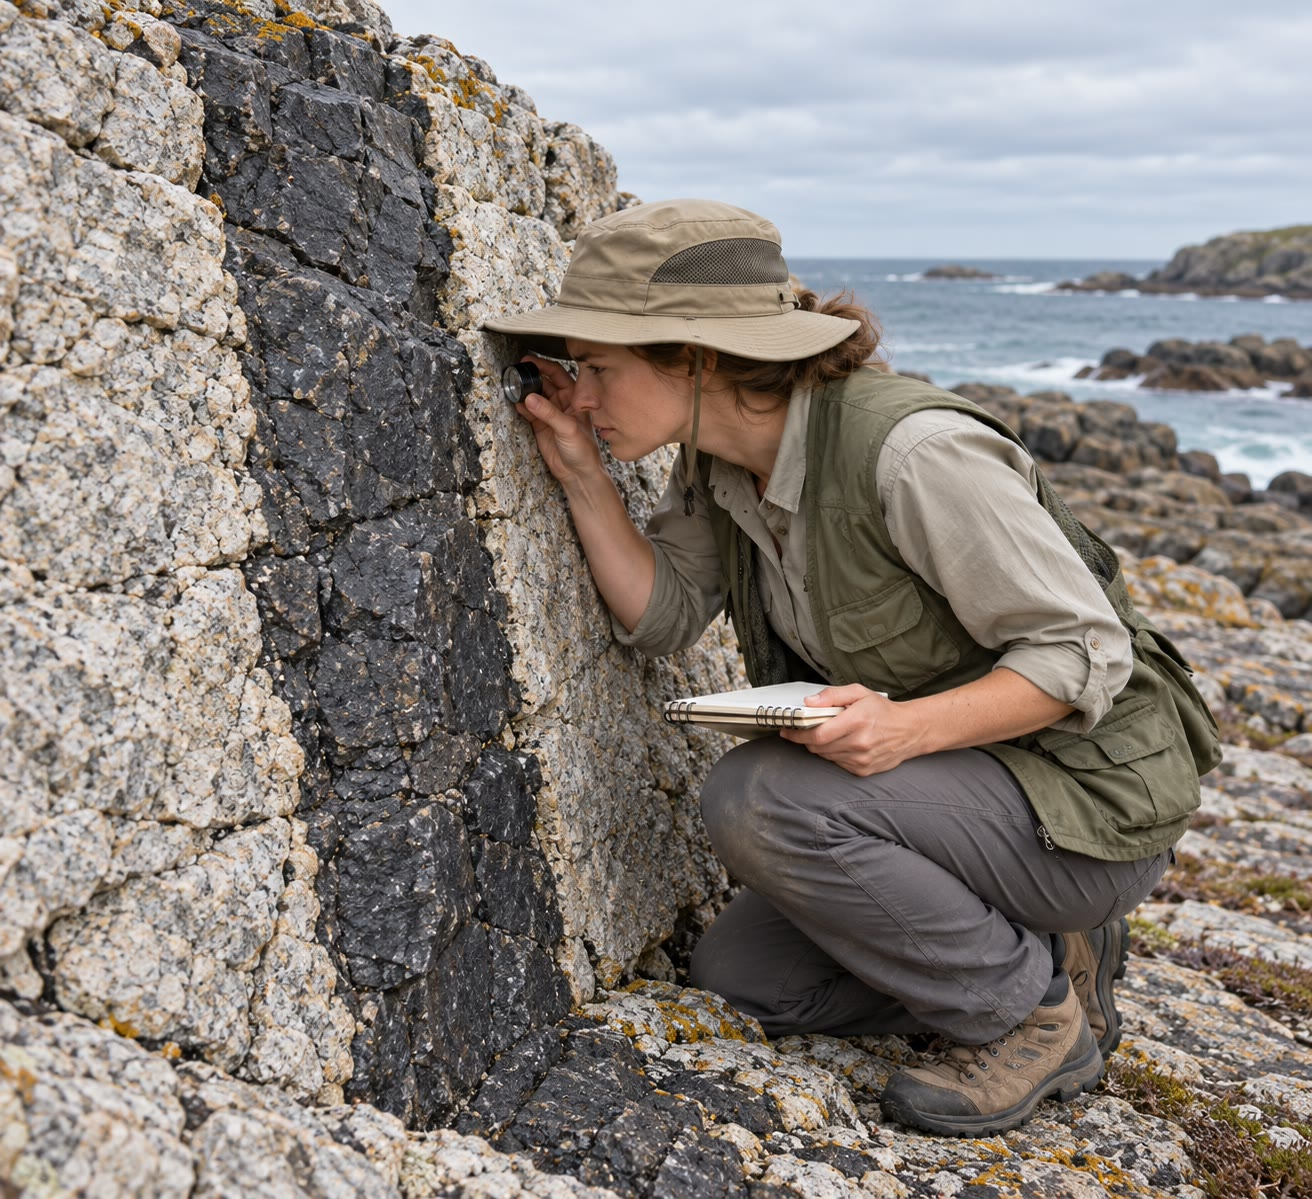
\includegraphics[width=\linewidth]{images/book4/ai/b2-dyke-contact.jpg}
\par\smallskip{\scriptsize جيولوجي يفحص تماس قاطع داكن مع
صخر مضيف فاتح (رسم توضيحي مولَّد بالذكاء الاصطناعي).}
\end{minipage}
\end{inthefield}
% ledger: earle:intrusive-bodies

\section{التمارين}

\begin{exercise}[$\star$]\label{exo:b2:magma-emplacement:1}
للمصاهير الغرانيتية المائية، تعطي معادلة مضبوطة على القياسات
$\log_{10}\eta = [-3.545 + 0.833\ln w] + [9601 - 2368\ln w]/\{T - [195.7 + 32.25\ln
w]\}$، حيث $\eta$ بوحدة \unit{Pa.s}، و$w$ المحتوى المائي بالنسبة المئوية الكتلية و$T$
بالكلفن. احسب $\log_{10}\eta$ عند \qty{800}{\celsius} من أجل $w = 1$ و$w = 4$،
والعامل الذي تُخفض به النسب المئوية الثلاث الإضافية من الماء اللزوجة.
\end{exercise}
% ledger: hd96:model

\begin{exercise}[$\star$]\label{exo:b2:magma-emplacement:2}
باستعمال قانون الجذر التربيعي، مع $s = 0.44$ للريوليت و$s = 0.34$ للبازلت
(نسبة مئوية كتلية لكل $\sqrt{\unit{MPa}}$)، احسب ضغط الإشباع لريوليت
فيه \qty{6}{\percent} من الماء ولبازلت فيه \qty{0.5}{\percent}،
والعمقين المقابلين في قشرة كثافتها \qty{2600}{kg/m^3}
($g = \qty{9.81}{m/s^2}$).
\end{exercise}

\begin{exercise}[$\star$]\label{exo:b2:magma-emplacement:3}
احسب درجة حرارة التماس لقاطع بازلتي عند \qty{1150}{\celsius}
اندسّ في صخور عند \qty{50}{\celsius}، ثم في صخور عند
\qty{400}{\celsius}. أيّ القاطعين ستكون حافته المبرّدة أعرض؟
\end{exercise}

\begin{exercise}[$\star$]\label{exo:b2:magma-emplacement:4}
سمِّ كل جسم. (أ) صفيحة من الدوليريت سمكها \qty{30}{m} تقع بين طبقتين
من الحجر الرملي على امتداد \qty{20}{km}. (ب) صفيحة رأسية من البازلت عرضها \qty{2}{m}
تقطع أحجارًا جيرية أفقية. (ج) غرانيت يتكشّف على مساحة \qty{2000}{km^2}،
مكوّن من دزينة وحدات مختلفة الأعمار. (د) عدسة من البورفيري قطرها \qty{1}{km}،
مسطّحة عند قاعدتها، تتقوّس فوقها الطبقات إلى الأعلى. (ه) صفيحة أفقية
من البازلت في غرانيت.
\end{exercise}

\begin{exercise}[$\star\star$]\label{exo:b2:magma-emplacement:5}
لمصهور بازلتي $\eta_{\ell} = \qty{100}{Pa.s}$. باستعمال علاقة أينشتاين وروسكو
($R = 1.35$)، احسب لزوجة \omterm{def:b2:magma-emplacement:magma}{الصهارة} التي فيها
\qty{5}{\percent} و\qty{20}{\percent} و\qty{40}{\percent} و\qty{60}{\percent} من
البلّورات، وقارن الأولى بصيغة أينشتاين للمعلّقات المخفّفة. عند أيّ حصّة من
البلّورات تتنبّأ العلاقة بالانحشار؟
\end{exercise}

\begin{exercise}[$\star\star$]\label{exo:b2:magma-emplacement:6}
تصعد صهارة كثافتها أقل من كثافة جدرانها بمقدار \qty{300}{kg/m^3} عبر قاطع.
(أ) لبازلت ($\eta = \qty{100}{Pa.s}$، $\rho = \qty{2700}{kg/m^3}$) في قاطع
عرضه \qty{1}{m}، احسب السرعة المتوسطة، والتدفّق لكل متر من \omterm{def:b2:magma-emplacement:bodies}{القاطع}،
وعدد رينولدز، وزمن الصعود \qty{10}{km}. (ب) الزمن نفسه لريوليت لزوجته
\qty{e6}{Pa.s} في قاطع عرضه \qty{1}{m}، ثم \qty{10}{m}. (ج) يفقد قاطع
عرضه \qty{1}{m} حرارته في زمن من رتبة $(w/2)^2/\kappa$، مع $\kappa =
\qty{1e-6}{m^2/s}$: أيّ الصعودات الثلاثة يمكن أن ينجح؟
\end{exercise}

\begin{exercise}[$\star\star$]\label{exo:b2:magma-emplacement:7}
تحرّر صهارة كثافتها \qty{2400}{kg/m^3} عند \qty{900}{\celsius}
\qty{1}{\percent} من كتلتها بخار ماء. باعتبار البخار غازًا مثاليًا
($R = \qty{8.314}{J/(mol.K)}$، \qty{18.015}{g/mol})، احسب الكسر الحجمي
للغاز في \omterm{def:b2:magma-emplacement:magma}{الصهارة} عند \qty{100}{MPa} و\qty{10}{MPa} و\qty{0.1}{MPa}. أيّ
القيم الثلاث أقلها موثوقية، ولماذا؟
\end{exercise}

\begin{exercise}[$\star\star$]\label{exo:b2:magma-emplacement:8}
في حوض، تزداد كثافة الصخور مع العمق $z$ وفق $\rho(z) =
2300 + 60\,z$ (\unit{kg/m^3}، و$z$ بوحدة \unit{km}) حتى \qty{10}{km}. (أ) أين يقع
\omterm{def:b2:magma-emplacement:ascent}{مستوى الطفو المتعادل} لمصهور بازلتي كثافته \qty{2650}{kg/m^3}؟ (ب) يُظهر
نموذج الكثافة في هذا الفصل أن واحدًا في المئة من الماء المذاب يُخفض
كثافة المصهور البازلتي بنحو \qty{70}{kg/m^3}. أين يتوقف مصهور فيه
واحد في المئة إضافي من الماء؟ (ج) ما قوة الطفو لكل متر مكعب
من المصهور الجاف على عمق \qty{2}{km} تحت مستوى طفوه المتعادل؟
\end{exercise}

\begin{exercise}[$\star\star$]\label{exo:b2:magma-emplacement:9}
لنفترض أن ديابيرًا غرانيتيًا نصف قطره \qty{1}{km} ونقص كثافته
\qty{300}{kg/m^3} يصعد عبر قشرة سفلى لزوجتها \qty{e19}{Pa.s}. احسب
سرعة ستوكس له (كرة صلبة) بالملّيمتر في السنة وزمن الصعود
\qty{10}{km}. وقارن بالسلّم الزمني $a^2/\kappa$ لتبريده، مع $\kappa
= \qty{1e-6}{m^2/s}$. ماذا تستنتج؟
\end{exercise}

\begin{exercise}[$\star\star\star$]\label{exo:b2:magma-emplacement:10}
يذوب الماء في مصهور على هيئة جزيئات، $x_m = K_1 f$، وعلى هيئة مجموعات
هيدروكسيل، $x_{\mathrm{OH}}^2 = K_2 x_m$ (وأكسجين المصهور بفائض كبير)، بحيث
يكون الماء المذاب الكلي $x = x_m + x_{\mathrm{OH}}/2$. (أ) عبّر عن $x$ بدلالة
$f$ وبيّن أنه يسلك سلوك $\sqrt f$ عند $f$ المنخفضة وسلوك $f$ عند
$f$ المرتفعة. (ب) عند أيّ فوغاسية يتساوى وفور شكلي الماء؟ (ج)
مع $K_1 = \qty{1e-4}{MPa^{-1}}$ و$K_2 = 0.2$، احسب هذه الفوغاسية،
وحصّة الماء المذاب على هيئة هيدروكسيل عند \qty{100}{MPa}.
\end{exercise}

\begin{exercise}[$\star\star\star$]\label{exo:b2:magma-emplacement:11}
يتجمّع بلوتون غرانيتي حجمه \qty{1000}{km^3} على مدى \qty{4}{Myr}. (أ) احسب
متوسط إمداده \omterm{def:b2:magma-emplacement:magma}{بالصهارة} بوحدة \unit{km^3} في السنة وبوحدة \unit{m^3} في الثانية. (ب)
يغذّيه قاطع واحد طوله \qty{1}{km} وعرضه \qty{2}{m}، سرعته المتوسطة
\qty{0.8}{m/s}: كم يستغرق \omterm{def:b2:magma-emplacement:bodies}{القاطع} لإيصال \omterm{def:b2:magma-emplacement:bodies}{البلوتون}
كله؟ وما الحصّة التي يمثّلها ذلك من \qty{4}{Myr}؟ (ج) إذا كان \omterm{def:b2:magma-emplacement:bodies}{البلوتون} مبنيًا من
صفائح سمكها \qty{20}{m} وأبعادها \qty{10}{km} في \qty{10}{km}، فكم صفيحة
يلزم، وكم من الزمن يفصل في المتوسط بين اثنتين منها؟ (د) مع
$\lambda = 0.65$ و$\kappa = \qty{0.7e-6}{m^2/s}$، كم تستغرق الصفيحة لكي
تتصلّب؟ هل كان \omterm{def:b2:magma-emplacement:bodies}{البلوتون} يومًا جسمًا كبيرًا واحدًا من \omterm{def:b2:magma-emplacement:magma}{الصهارة}؟
\end{exercise}

\begin{exercise}[$\star\star\star$]\label{exo:b2:magma-emplacement:12}
بعيدًا عن قاطع رقيق عرضه $b$ (على مسافات $x \gg b$)، تعمل حرارته كمصدر
مستوٍ لحظي: $T - T_0 = (T_m - T_0)\,b\,e^{-x^2/(4\kappa
t)}/\sqrt{4\pi\kappa t}$. (أ) بيّن أن درجة الحرارة على المسافة $x$ تبلغ أقصاها عند
$t^* = x^2/(2\kappa)$، وأن هذا الارتفاع الأقصى هو $\Delta T_{\max} = (T_m -
T_0)\,b/(x\sqrt{2\pi e})$. (ب) لقاطع عرضه \qty{2}{m} مع $T_m - T_0 =
\qty{1100}{K}$، على أيّ مسافة يسخن الصخر بمقدار \qty{100}{K} على الأكثر،
ومتى ($\kappa = \qty{0.7e-6}{m^2/s}$)؟ (ج) لماذا تكون هالات القواطع الرقيقة
ضيّقة إلى هذا الحدّ؟
\end{exercise}

\section{مسألة: العتبة تحت الهضبة}

\begin{problem}[{مسألة نهاية الأسبوع --- تتبّع صهارة بازلتية من قاطعها المغذّي
إلى عتبة، وماؤها، والزمن الذي تستغرقه العتبة لتتصلّب}]
\label{pb:b2:magma-emplacement:1}
تحت هضبة متخيَّلة، ترتكز رسوبيات (طفل وحجر رملي) متوسط كثافتها
\qty{2450}{kg/m^3} على عمق \qty{3.0}{km} فوق قاعدة بلّورية
كثافتها \qty{2800}{kg/m^3}. صعدت صهارة بازلتية من \qty{15}{km} عبر قاطع
عرضه \qty{2.0}{m} وانتشرت على امتداد قاعدة الرسوبيات عتبةً من الدوليريت
سمكها \qty{100}{m}. البيانات: درجة حرارة الاندساس \qty{1150}{\celsius}؛ قانون لزوجة
المصهور $\log_{10}\eta = -4.55 + 5510/(T - 611)$ ($T$ بالكلفن)؛ كثافة
المصهور مع مائه \qty{2710}{kg/m^3}؛ \qty{20}{\percent} من البلّورات حجمًا
(أينشتاين وروسكو، $R = 1.35$)؛ الماء المذاب \qty{0.40}{\percent}، والذوبانية
$s = 0.34$ في المئة لكل $\sqrt{\unit{MPa}}$؛ درجة حرارة المضيف عند \omterm{def:b2:magma-emplacement:bodies}{العتبة}
\qty{100}{\celsius}؛ $\kappa = \qty{0.7e-6}{m^2/s}$، $\rho c = \qty{2.5}{MJ/(m^3.K)}$،
الحرارة الكامنة \qty{900}{MJ/m^3}، مع اعتبار \omterm{def:b2:magma-emplacement:magma}{الصهارة} تتصلّب عند درجة حرارة
اندساسها؛ $g = \qty{9.81}{m/s^2}$؛ والسنة الواحدة \qty{3.156e7}{s}.

\medskip\noindent\textbf{الجزء الأول --- \omterm{def:b2:magma-emplacement:magma}{الصهارة}.}
\begin{enumerate}
\item احسب $\log_{10}\eta$ و$\eta$ للمصهور عند \qty{1150}{\celsius}
(\qty{1423}{K}).
\item السؤال نفسه عند \qty{1100}{\celsius}. بأيّ عامل تتغيّر اللزوجة على
هذه الدرجات الخمسين (\qty{50}{K})؟
\item احسب لزوجة \omterm{def:b2:magma-emplacement:magma}{الصهارة} مع بلّوراتها عند
\qty{1150}{\celsius}.
\item عند أيّ حصّة من البلّورات تجعل علاقة أينشتاين وروسكو
\omterm{def:b2:magma-emplacement:magma}{الصهارة} تنحشر؟ قارن بالتقدير الحقلي لنهاية الجريان الكلي.
\item احسب فرق الكثافة بين \omterm{def:b2:magma-emplacement:magma}{الصهارة} والقاعدة،
وبين \omterm{def:b2:magma-emplacement:magma}{الصهارة} والرسوبيات.
\item احسب الضغط الصخري عند مستوى \omterm{def:b2:magma-emplacement:bodies}{العتبة}.
\end{enumerate}

\noindent\textbf{الجزء الثاني --- صعودًا في \omterm{def:b2:magma-emplacement:bodies}{القاطع}.}
\begin{enumerate}[resume]
\item احسب تدرّج ضغط الطفو $\Delta\rho\,g$ الذي يدفع \omterm{def:b2:magma-emplacement:magma}{الصهارة}
عبر القاعدة.
\item احسب السرعة المتوسطة للصهارة في \omterm{def:b2:magma-emplacement:bodies}{القاطع}.
\item احسب التدفّق لكل متر من \omterm{def:b2:magma-emplacement:bodies}{القاطع}، والتدفّق الكلي إذا كان طول \omterm{def:b2:magma-emplacement:bodies}{القاطع}
\qty{1.0}{km}.
\item احسب عدد رينولدز للجريان. هل هو صفائحي؟
\item كم تستغرق \omterm{def:b2:magma-emplacement:magma}{الصهارة} لتصعد من \qty{15}{km} إلى \qty{3.0}{km}؟
\item قارن بالسلّم الزمني $(w/2)^2/\kappa$ الذي يفقد فيه \omterm{def:b2:magma-emplacement:bodies}{القاطع}
حرارته. هل يستطيع أن يبقى مفتوحًا؟
\item اشرح لماذا توقفت \omterm{def:b2:magma-emplacement:magma}{الصهارة} عند \qty{3.0}{km} وانتشرت جانبيًا، مستعملًا
مفردات الفصل.
\end{enumerate}

\noindent\textbf{الجزء الثالث --- الماء.}
\begin{enumerate}[resume]
\item احسب ضغط الإشباع لماء المصهور، والعمق في
الرسوبيات الذي يُبلغ عنده.
\item ما كمية الماء التي يستطيع المصهور حملها عند مستوى \omterm{def:b2:magma-emplacement:bodies}{العتبة}؟ هل تفصل صهارة
\omterm{def:b2:magma-emplacement:bodies}{العتبة} ماءً؟
\item تحوي الحويصلات في \omterm{def:b2:magma-emplacement:aureole}{الحافة المبرّدة} للعتبة أساسًا CO$_2$. اشرح.
\item لو خرج كل الماء البالغ \qty{0.40}{\percent} عند السطح، عند
\qty{1150}{\celsius} و\qty{0.1}{MPa}، فما الكسر الحجمي من \omterm{def:b2:magma-emplacement:magma}{الصهارة} الذي
يشغله البخار (غاز مثالي)؟
\end{enumerate}

\noindent\textbf{الجزء الرابع --- التبريد والتصلّب.}
\begin{enumerate}[resume]
\item بإهمال الحرارة الكامنة، احسب درجة حرارة التماس للعتبة.
\item بإهمال الحرارة الكامنة، احسب درجة الحرارة على بعد \qty{10}{m} فوق التماس
العلوي بعد \num{10}~سنوات من الاندساس.
\item النموذج نفسه: احسب درجة الحرارة في منتصف \omterm{def:b2:magma-emplacement:bodies}{العتبة} بعد
\num{10}~سنوات و\num{50}~سنة.
\item النموذج نفسه: على بعد \qty{80}{m} فوق التماس العلوي، احسب درجة الحرارة بعد
\num{300} و\num{363} و\num{420} سنة. هل تبلغ الصخور هناك يومًا
\qty{300}{\celsius}؟
\item احسب $L\sqrt\pi/(\rho c\,(T_m - T_0))$ للعتبة.
\item احسب قيمة $e^{-\lambda^2}/(\lambda(1 + \operatorname{erf}\lambda))$ من أجل $\lambda = 0.64$
و$0.65$ و$0.66$ ($\operatorname{erf}0.64 = 0.6346$، $\operatorname{erf}0.65 = 0.6420$،
$\operatorname{erf}0.66 = 0.6494$)، وأعطِ $\lambda$ بمنزلتين عشريتين.
\item مع الحرارة الكامنة، احسب درجة حرارة التماس أثناء تصلّب
\omterm{def:b2:magma-emplacement:bodies}{العتبة}. لماذا هي أعلى منها في السؤال 18؟
\item احسب السلّم الزمني $(b/2)^2/\kappa$ بالسنوات.
\item احسب الزمن الذي تستغرقه \omterm{def:b2:magma-emplacement:bodies}{العتبة} لتتصلّب، بالسنوات، وهو الرقم الأساسي في
هذه المسألة، واشرح لماذا هو أقصر من السلّم الزمني في السؤال
السابق مع أن الحرارة الكامنة يجب أن تُزال.
\end{enumerate}
\end{problem}
% ledger: grd08:model, kolz22:einstein-roscoe, glazner04:tuolumne, moore98:h2o, lowenstern01:co2, delaney86b4:properties
